\documentclass{article}
\usepackage[utf8]{inputenc}
\usepackage{graphicx}
\usepackage{caption}
\usepackage{multicol}
\usepackage{amsmath}
\usepackage[left=1cm,right=1cm,top=2cm]{geometry}


\usepackage{esvect}
\usepackage{latexsym}

\usepackage{url}


\title{A Concise Report of Machine Learning's Project\\\large{First Milestone : Data }}
\author{Zahra Farahmand, Reyhaneh Aghaei, Bahar Nikbakht}
\date{March 2020}

\begin{document}

\maketitle

In this report, which is aimed mostly the aspects of the data, we have explained briefly about the whole project, the method we have used for generating data and the general features of Cosmic Microwave Background.Then we have clarified the different types of precision we may face on during the project, and at the end, we have named some of the related articles.

\begin{multicols}{2}

\section{Introduction}
According to inflation theory, the speed of propagation of quantum fluctuations in the early universe is not necessarily equals to the speed of light. This makes it sounds sensible to think of cherenkov effect, in which a particle goes beyond the speed of sound and though the trace of it's path will remain in the surroundings,just like mach cones made by ultrasonic airplanes in the sky. On the other hand, due to a recent claim, massless particles may have intersected the horizon and made the same cones due to the speed of propagation of quantum fluctuations (hereinafter called $C_s$) and the cherenkov effect as a result \cite{claim}.

On the other hand, Cosmic Microwave Background (CMB) remaining from the era when the universe was young, could be used as a snapshot of the whole universe which involves these traces.However CMB is too dense to look forward special shapes on it without the help of machine learning's methods.On the first step of this project we are going to portrait the general shapes of the traces on the CMB, and find a proper method of simulating them in order to be used in further training.

\section{Cone-Sphere Intersection}

As mentioned above, the traces of the massless particles on CMB,which is seems spherical to us, are in different shapes that a cone-sphere intersection may have (Figure \ref{fig:fig1}).

The cone-sphere intersections are various in shape.it made us to look for a general function which enables us to know whether a point is on the intersection or not.
\subsection{General Solution to Cone-Sphere Intersections}
First, consider a sphere at the origin with unit radius, actually the length of the radius doesn't matter, we should just take care that every distance should be normalized by our distance to CMB.

\hspace{-0.5cm}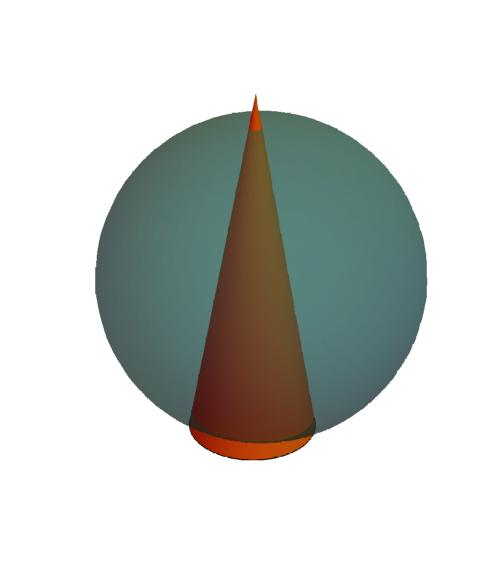
\includegraphics[width=0.15\textwidth]{I1.jpg}
\hspace{-0.5cm}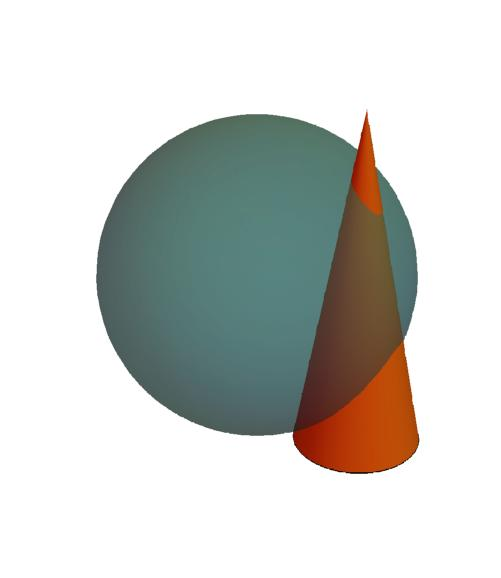
\includegraphics[width=0.15\textwidth]{I3.jpg}
\hspace{-0.5cm}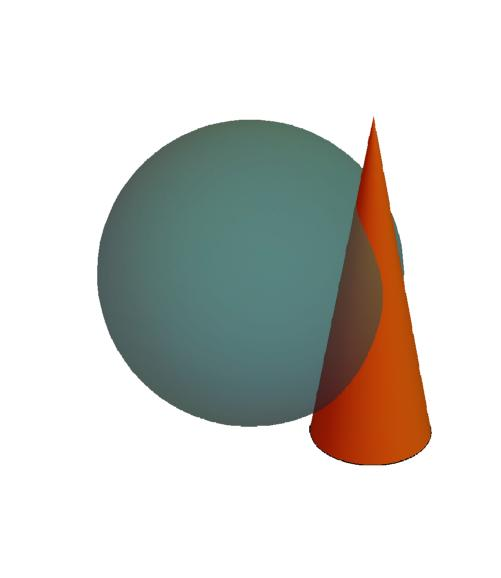
\includegraphics[width=0.15\textwidth]{I4.jpg}
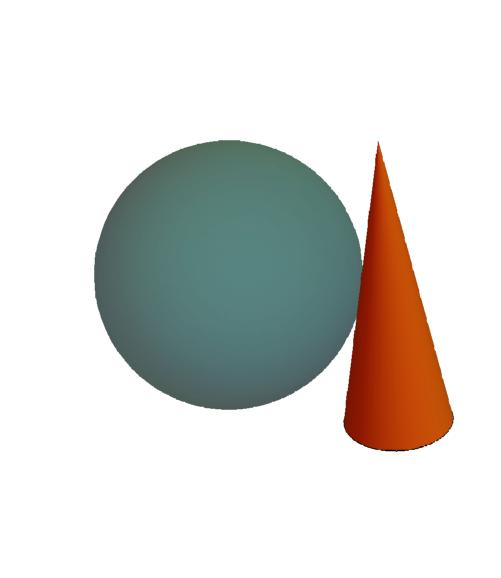
\includegraphics[width=0.15\textwidth]{I5.jpg}
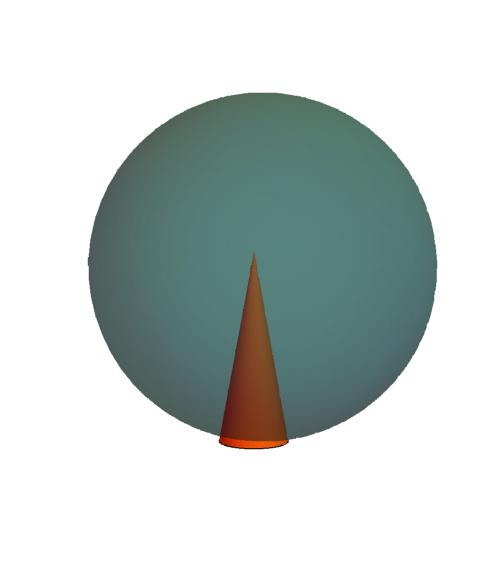
\includegraphics[width=0.15\textwidth]{I6.jpg}
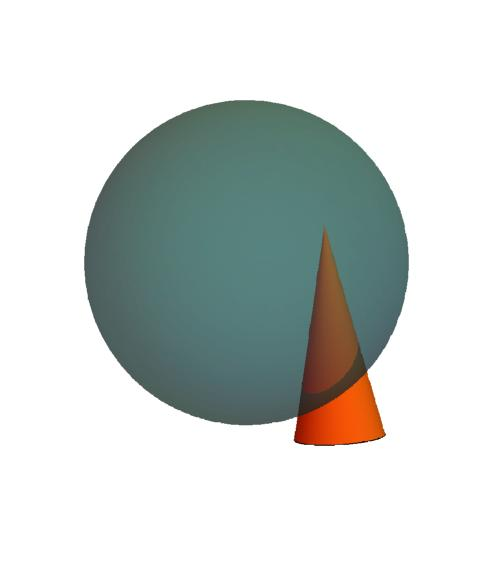
\includegraphics[width=0.15\textwidth]{I8.jpg}
\captionof{figure}{Probable shapes of cone-sphere intersections}
\label{fig:fig1}
\medskip

Then imagine a cone with angle $\theta_{C_s}$, a head positioned at $\vv{r_0}$ and a direction vector $\vv{n}$, which crosses the sphere (Figure \ref{fig:cherenkov}).

\hspace{+2cm}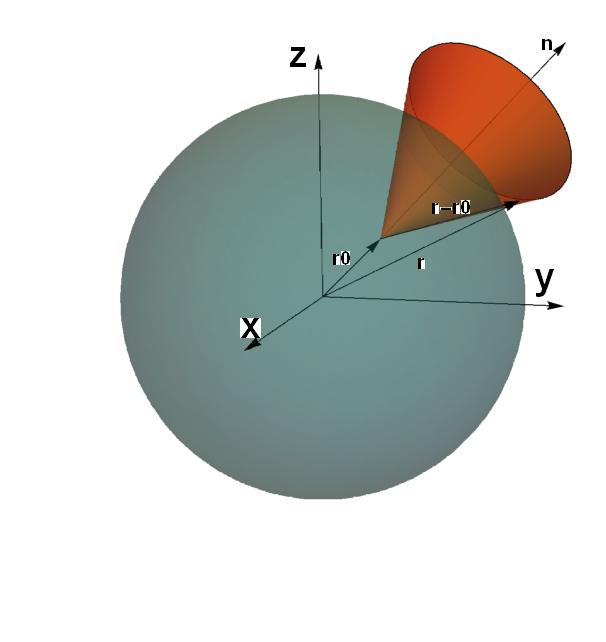
\includegraphics[width=0.3\textwidth]{cherenkov.jpg}
\captionof{figure}{intersection of a sphere and a cone}
\label{fig:cherenkov}

The parameters of the cone are expressed as:
\begin{align}
\vv{r_0} = x_0 \hat{x} + y_0 \hat{y} + z_0 \hat{z},
\\
\vv{n} = n_x \hat{x} + n_y \hat{y} + n_z \hat{z}. 
\end{align}

A cone in general can be defined as a locus of  all vectors with the same angle relative to a single vector.here, the single vector which we are looking for is $\vv{n}$. So, by using the relation between the magnitude of the product of dot operator and the magnitude of the vectors themselves, the general cone equation can be written as follows:
\begin{align}
(\vv{r}-\vv{r_0}) \cdot \vv{n} = |\vv{r}-\vv{r_0}| \cos{\theta_{C_s}}.
\end{align}
By using the above equation and equations (1) and (2), and considering $r=X\hat{x}+Y\hat{y}+Z\hat{z}$ we have:
\begin{align}
(X-x_0)n_x+(Y-y_0)n_y+(Z-z_0)n_z = |\vv{r}-\vv{r_0}| \cos{\theta_{C_s}}.
\label{Eq:equation1} %the label lets you refer to the equation later
\end{align}
Intersection points($\{\theta^{*},\phi^{*}\}$) must satisfy both equations of the cone and the sphere,so they can be represented by the following system of equations,
\begin{gather*}
   \vv{r}^{*}(\theta^{*},\phi^{*}) = R(\sin{\theta^{*}} \cos{\phi^{*}}\hat{x} + \sin{\theta^{*}} \sin{\phi^{*}} \hat{y} + \cos{\theta^{*}} \hat{z}) ,
   \\
   (\vv{r}^{*}-\vv{r_0}) \cdot \vv{n} = |\vv{r}^{*}-\vv{r_0}| \cos{\theta_{C_s}}.
   \label{Eq:equation1} %the label lets you refer to the equation later
\end{gather*}

\subsection{Cone-Sphere Intersection Data}
By solving the system of equations obtained in the previous subsection, the general equation of the intersection points would be:
\begin{multline}
       f(\theta,\phi) = (\sin{\theta} \cos{\phi} - x_0) n_x + (\sin{\theta} \sin{\phi}- y_0) n_y\\ + (\cos{\theta} - z_0) n_z - \cos{\theta_{C_s}} \bigg((\sin{\theta} \cos{\phi} - x_0)^2 \\ + ( \sin{\theta} \sin{\phi}- y_0)^2 + (\cos{\theta} - z_0)^2\bigg)^{\frac{1}{2}} = 0 .
\end{multline}

We aim to use simulation for generating intersection curves' data with the same format as the CMB data, in which the space is discreted to pixels and each pixel contains the magnitude of the temperature of that pixel (see section 3.1).To solve the equation(5) numerically, parameters $\theta$ and $\phi$ of the space should be discreted. 

In order to simulate the two dimensional matrix(intersection matrix) that the nonzero elements’ position stand for intersection’s $\{\theta,\phi\}$, we divide parameter space into $N_{\theta}\times N_{\phi}$ parts(Figure \ref{fig:parameter space}).
\begin{equation*}
    N_{\theta} = \frac{\pi}{\Delta \theta}\;\;\;N_{\phi} = \frac{2\pi}{\Delta \phi},
\end{equation*}
\begin{multline}
   function\: matrix = F = \sum_{i,j}^{N_{\theta},N_{\phi}} F_{i,j} = \sum_{i,j}^{N_{\theta},N_{\phi}} f({\theta_i,\phi_j}).
\end{multline}

Which $\Delta \theta$ and $\Delta \phi$ are the CMB’s precision of $\theta$ and $\phi$.

\hspace{+1.5cm}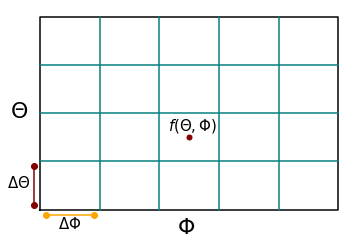
\includegraphics[width=0.3\textwidth]{download.png}
\captionof{figure}{schematic diagram of discrete parameter space}
\label{fig:parameter space}
\medskip
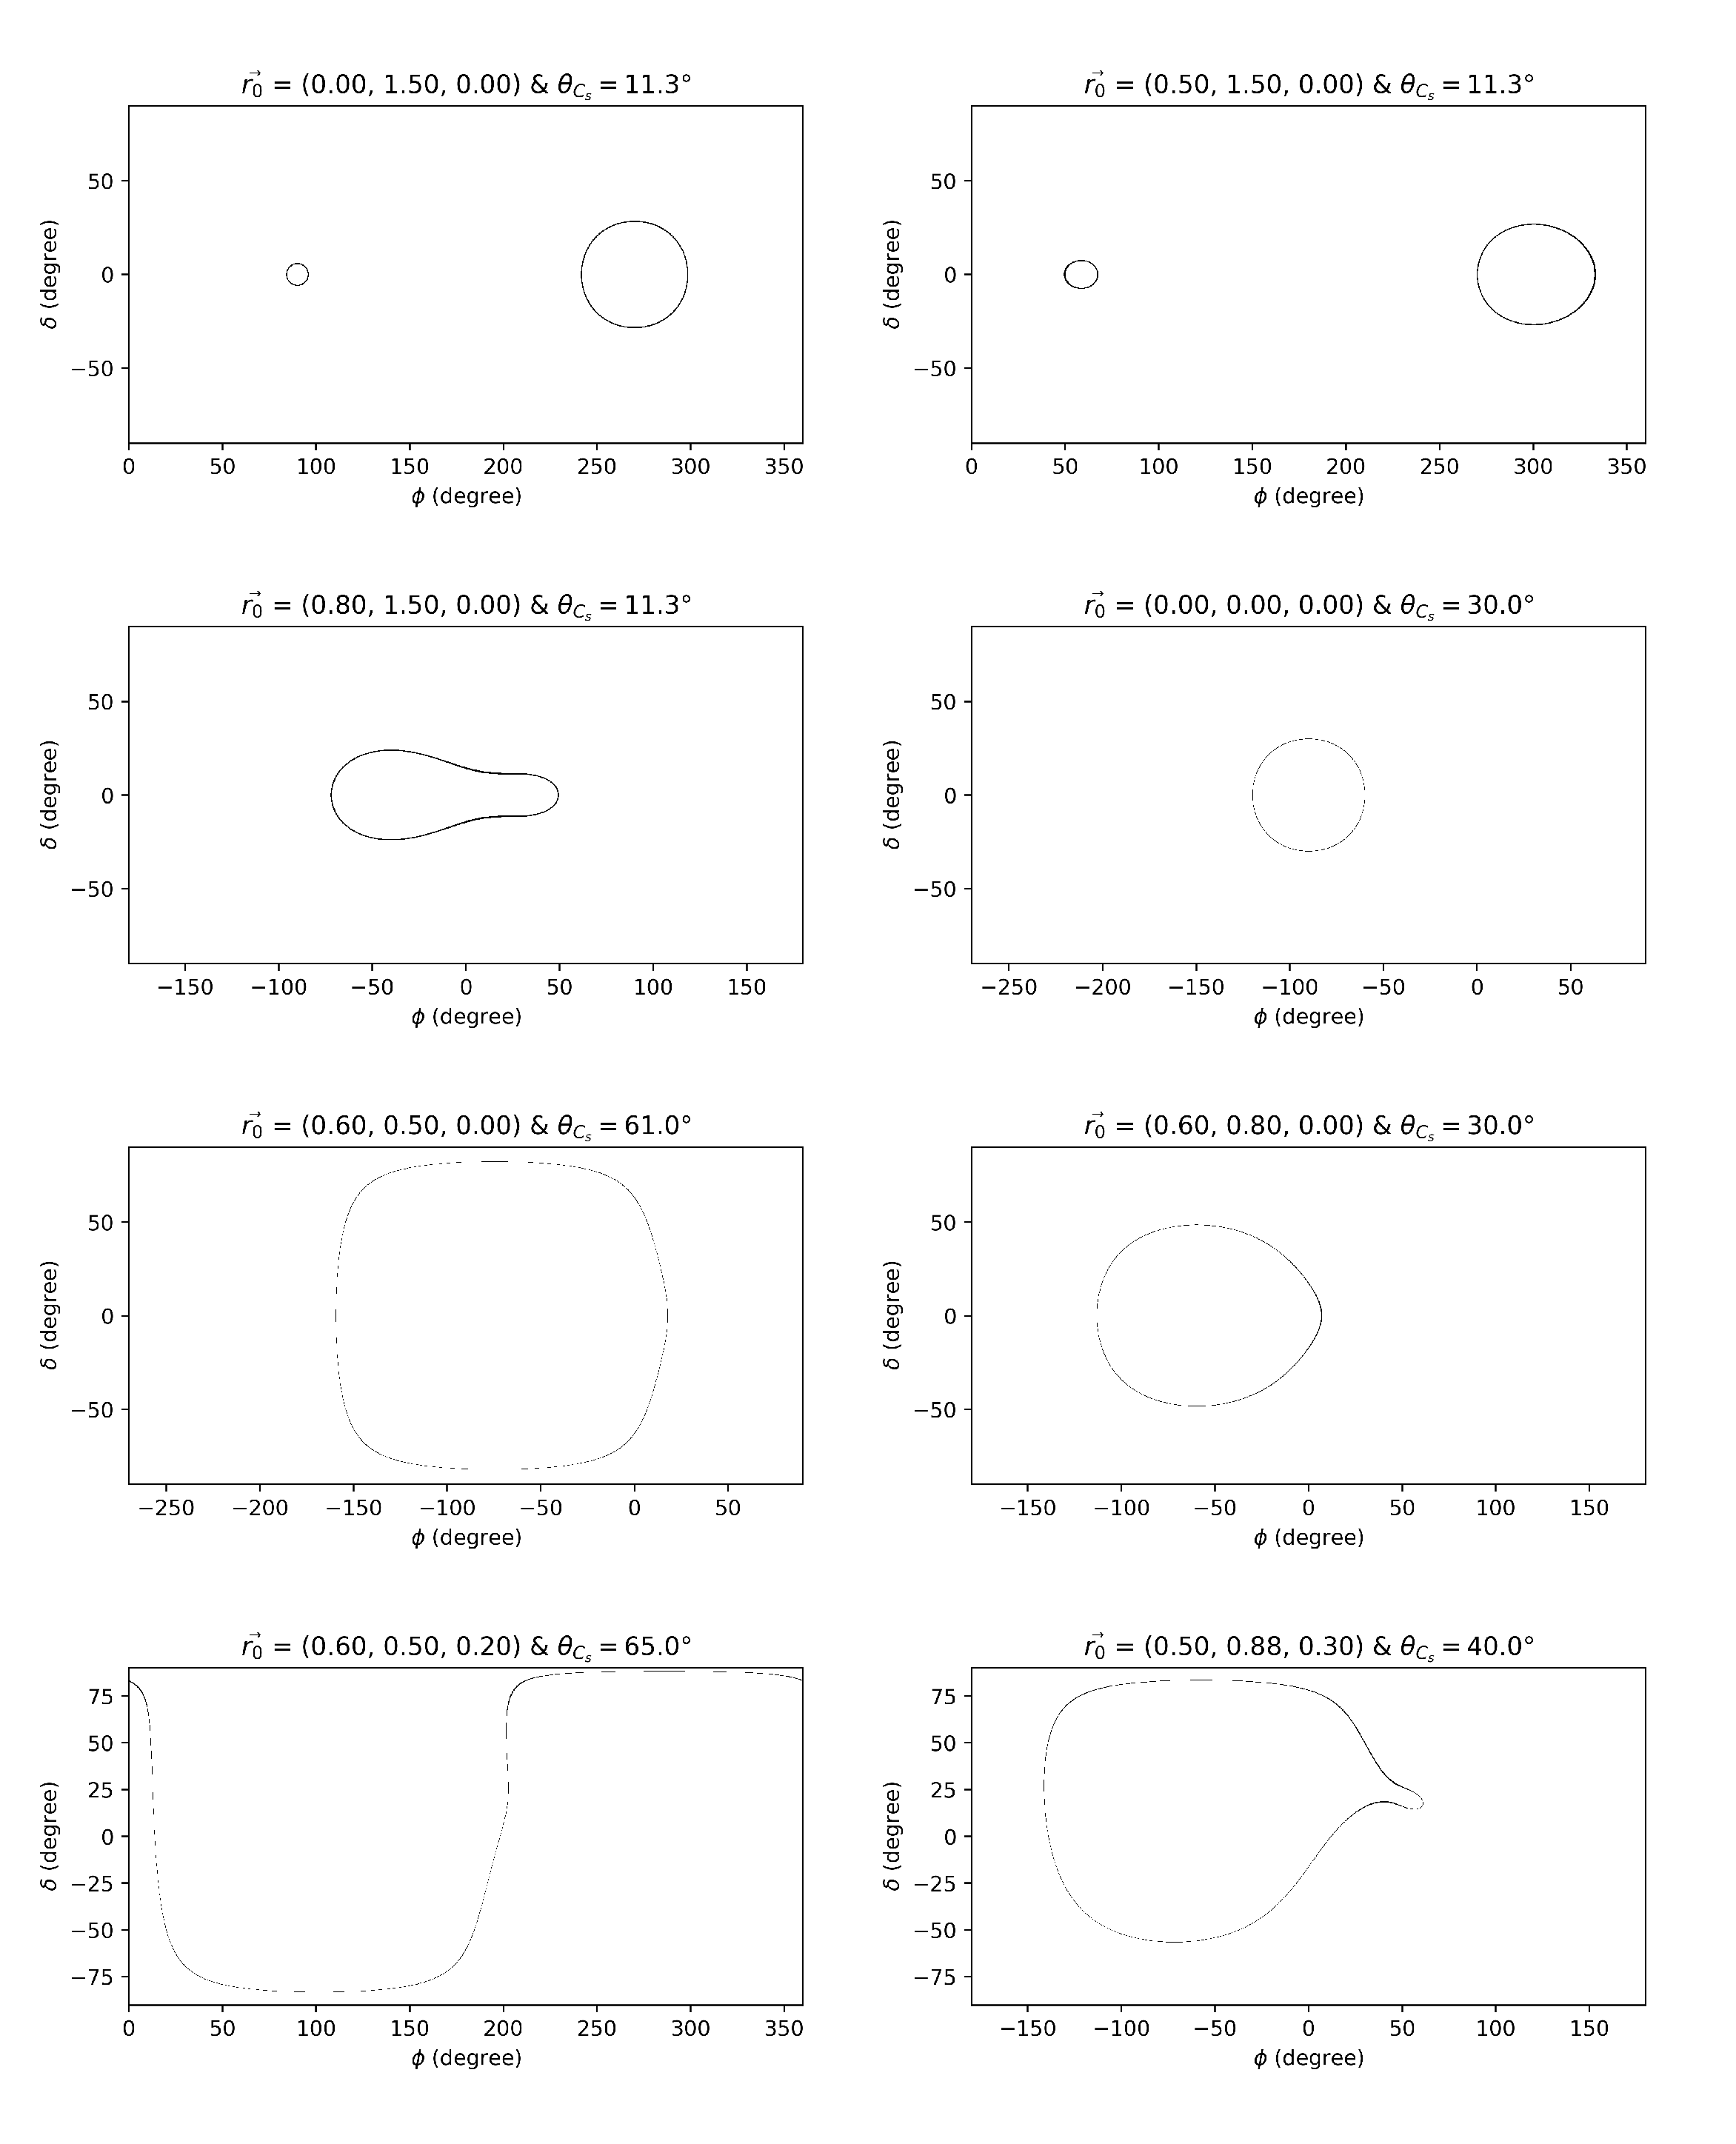
\includegraphics[width=0.5\textwidth]{image.png}
\captionof{figure}{different curves for cones with (0,-1,0) direction vector}
\label{fig:sample}
\medskip
Due to discrete parameters considering an error becomes a fundamental issue.We need a threshold for flagging each of function matrix elements as an intersection point and create intersection matrix. Two different ways are tested:
\begin{enumerate}
\item
Consider an error matrix($F_{error}$) with same dimension as function matrix and compare $F_{i,j}$ with ${F_{error}}_{i,j}$ for finding corresponding intersection matrix elements.
\begin{equation}
   \Delta f(\theta , \phi) = \sqrt{ (\frac{\partial f}{\partial \theta} \Delta \theta)^2 + (\frac{\partial f}{\partial \phi} \Delta \phi)^2}\;.
   \label{Eq:equation1} %the label lets you refer to the equation later
\end{equation}
\item
According to the precision of the physical aspects of the problem,set a constant error to compare function matrix elements with it. 
\end{enumerate}

Till now, we have succeeded finding a firm framework of generating data, in which we use $\vv{n}$, $\vv{r_0}$ and $\theta_{C_s}$ as inputs ,and the output is a matrix of meshed space,as mentioned before, with one elements on the intersection line and zero in other parts of the space. however, still some minor issues have remained unsolved. We are not sure about the intervals in which the parameters vary, hence this is concerned with the physical aspects of the problem, and we are not sure about how many data sets would be sufficient for training. We are going to find an accurate answer to these problems meanwhile the next step.

\section{CMB Data}
The European Space Agency’s Planck satellite, which was dedicated to studying the early Universe and its subsequent evolution, observing the whole sky for nearly nine years,have equipped us with the precise map of the Cosmic Microwave Background, Known as CMB.Analysis of the Planck 2018 data set indicates that the statistical properties of the cosmic microwave background (CMB) temperature anisotropies are in excellent agreement with previous studies using the 2013 and 2015 data releases, proving that sky is isotropic as was expected before \cite{planck1}.

As mentioned in the previous sections,we are going to look forward to the cone-sphere intersections through temperature map of CMB. In this section, we are going to review one of the common methods of studying CMB, then explaining the method of cleaning the data, and a brief description of data's statistics and accuracy.

\subsection{Analysis of Data Distributed on the Sphere}
The Hierarchical Equal Area iso-Latitude Pixelization, or HEALPix in short, is a versatile data structure with an associated library of computational algorithms which was first developed to address the data processing and analysis needs of the present generation of cosmic microwave background experiments \cite{healpix}. 

HEALPix may be seen as a division of the sphere into 12 base pixels (Figure \ref{fig:fig3}\footnote{credit:libguides.rhul.ac.uk/referencing/latex}) which are then subdivided to give the desired resolution. The amount of subdivision is given be the NSIDE number where NSIDE is always a power of 2 hence 1,2,4,8,16,32 etc. NSIDE specifies the number of subdivisions in each side of a base pixels, eg. for NSIDE=2, each of the 12 base pixels are subdivided into 4 parts (Figure \ref{fig:fig4}\footnote{credit:libguides.rhul.ac.uk/referencing/latex}).
in the case of CMB Data which we are going to use, NSIDE=2048 so the total number of pixels is,
\begin{equation}
    N_{pix} = 12\times NSIDE^2 = 12\times 2048^2 = 50331648 .
\end{equation}

\hspace{+1.8cm}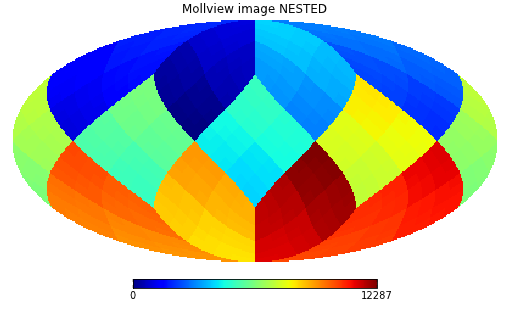
\includegraphics[width=0.32\textwidth]{moll_nside32_nest.png}
\captionof{figure}{12 HEALPix base pixels}
\label{fig:fig3}

\hspace{+1.8cm}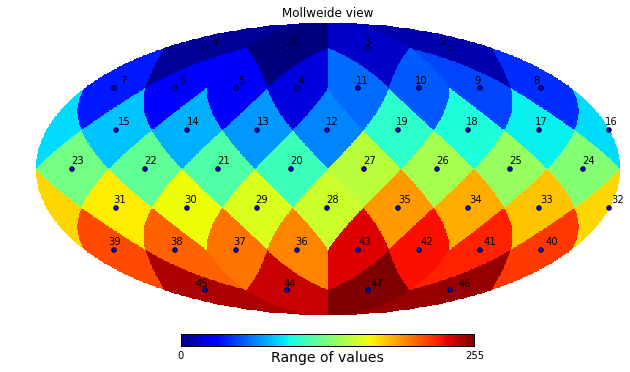
\includegraphics[width=0.32\textwidth]{index.png}
\captionof{figure}{Subdivisions of HEALPix pixels for NSIDE=2}
\label{fig:fig4}
\medskip

By using HEALPix library, the data can be easily reshape to the form of galactic coordinates and then represent by an array with indices $\theta$ and $\phi$ and the temperature in each element, the same as the format we have used for the results of the simulation of the cone-sphere intersections.The Inpainted I intensity map of the 2018 release of Planck data \footnote{Data are taken from Planck's website : pla.esac.esa.int} can be shown as Figure \ref{fig:CMB}.

The histogram of the difference of above data from it's mean is shown in Figure \ref{fig:hist}, showing that the temperature distribution of the universe is gaussian, in agreement with homogeneity and isotropy.

\hspace{+1cm}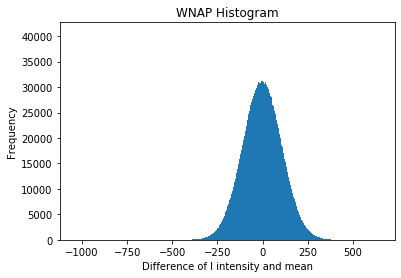
\includegraphics[width=0.33\textwidth]{hist.png}
\captionof{figure}{Histogram of the difference of the temperature map of Planck data (2018) and it's mean.}
\label{fig:hist}

\subsection{Method of Cleaning}
Planck detector, like all other CMB detectors that was used before, is a radio detector which counts the number of photons reaching it's CCD. The universe is almost empty making this process precise, however, our position in galactic disk cause the loss of some data, between $\theta=-18\deg$ to $\theta=+18\deg$.One of the most popular methods \footnote{A complete list of methods can be found here:$wiki.cosmos.esa.int/planckpla/index.php/CMB\_and\_astrophysical\_component\_maps$}that is used in order to clean up the CMB data, is SMICA. SMICA produces a CMB map by linearly combining all Planck input channels (from 30 to 857 GHz) with weights which vary with the multipole. It is a precise method but it's not necessary to keep these data until the end, we can easily throw them away at last, just as the same procedure done by Penrose and Gurzadyan\cite{ring}.

\section{Precision Considerations}
There are three types of precision which we must take care of:
\begin{enumerate}
\item
First of all we have to decide whether a pixel in CMB stands for a point or not, in other words, we should define a bound for temperature to divide the points of the shapes from the background.

\item
Second is the precision of the CMB itself, which bounded us for getting closer than a certain amount to a line which we expect to see and can be determined by the precision of $\theta$ and $\phi$.

\item
Finally,the precision of the traces that specifies the thickness of the lines we are looking for.This precision is straightly connected with the precision of $\theta_{C_s}$, that is the angle of the cone.

\end{enumerate}
The above types of precision, are somehow connected to each other.if the CMB resolution is not  sufficient, we won't be able to recognize the contrast between a target pixel region and the background.

As mentioned in section 2.1, we have pursuit two different approaches of precision, by calculating the exact amount of precision in each point and by considering a unit amount of precision in all space. The first approach that is much more precise costs the loss of speed. So, depending on the precision we may have to use in next spaces, we will choose what method to use.

\section{Related Articles}
In this section we are going mention some papers that are relevant to our project, with a small description of their relevance.

\begin{enumerate}
\item
A. A. Abolhasani and S. Jazayeri, “Cherenkov radiation in the sky:  Measuring the sound speed of primordial scalar fluctuations”

This is the main article that we are going to check it's validity. Although it's harder to comprehend by detail, but it may help us with the physics behind the whole story.

\item 
V. G. Gurzadyan, R. Penrose, "CCC-predicted low-variance circles in CMB sky and LCDM, " :

In this article, Gurzadyan and Penrose have done nearly the same thing. otherwise, they have searched for rings instead of cone-sphere intersections. and have done some statistical analysis that we can keep eye on them.

\item
C. L. Bennett, R. S. Hill, G. Hinshaw and others, "Seven-Year Wilkinson Microwave Anisotropy Probe (WMAP) Observations: Are There Cosmic Microwave Background Anomalies?" :

The above article have examined some of the statistical analysis of finding features and claiming that they are due to the non-standerd cosmology. it can help to provide a firm prof of what we find, if there is any!

\item
Planck Collaboration, "Planck 2018 results. I. Overview and the cosmological legacy of Planck"

This is the first article of a series of articles written by the Planck Collaboration, explaining the data of the Planck satellite and a complete analysis of it. It can be used to define a proper bound for the first type of precision mentioned above, and it can give us a sight of cleaning the data around the galactic disk.

\item
K. M. Gorski, E. Hivon, A. J. Banday, B. D. Wandelt, F. K. Hansen, M. Reinecke, M. Bartelman, "HEALPix -- a Framework for High Resolution Discretization, and Fast Analysis of Data Distributed on the Sphere"

The general method of HEALPix is clarified in this article then it allows us to use this library more efficiently.

\item
 Calabretta, Mark R., Roukema, Boudewijn F., "Mapping on the HEALPix grid "
 
 This paper is just the same as the above article, with some extra explanations about the position of each pixel in HEALPix.So, it can be used in the last part of the project to mark the excat pixels of CMB on the cone-sphere intersections' lines.
 
\item
 Amit Mishra, Pranath Reddy, Rahul Nigam, "CMB-GAN: Fast Simulations of Cosmic Microwave background Anisotropy maps using Deep Learning"
 
If we succeed in finding any cone-sphere intersections, the next step would be to show that this observation is due to non-standard cosmology, so we should run our models on virtual CMB's simulated by the standard model and compare the frequency of features.This article is about simulating CMB.

\item
Ali Frolop, Douglas Scott, "Pi in the sky":

It's about the same problem discussed in the article number 2, just  in shorter form.

\end{enumerate}


\end{multicols}

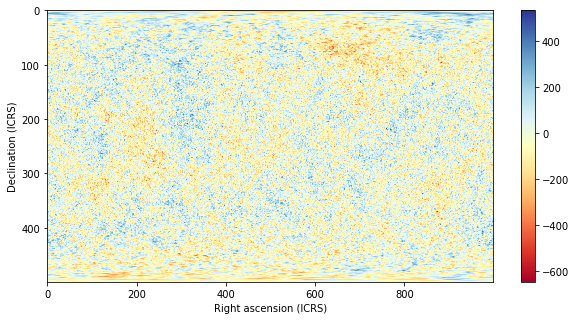
\includegraphics[width=1\textwidth]{cmb.png}
\captionof{figure}{CMB I Intensity map by Planck Data (2018)}
\label{fig:CMB}

\begin{thebibliography}{99}



\bibitem{claim} A. A. Abolhasani and S. Jazayeri, “Cherenkov radiation in the sky:  Measuring the sound speed of primordial scalar fluctuations,”Phys. Rev.D100no. 2, (2019) 023520,arXiv:1904.05589[astro-ph.CO].
\bibitem{planck1} Planck Collaboration, "Planck 2018 results. I. Overview and the cosmological legacy of Planck, "arXiv:1807.06205 [astro-ph.CO].
\bibitem{healpix}K. M. Gorski, E. Hivon, A. J. Banday, B. D. Wandelt, F. K. Hansen, M. Reinecke, M. Bartelman, "HEALPix -- a Framework for High Resolution Discretization, and Fast Analysis of Data Distributed on the Sphere" , 	Astrophys.J.622:759-771,2005,arXiv:astro-ph/0409513.
\bibitem{ring}V. G. Gurzadyan, R. Penrose, "CCC-predicted low-variance circles in CMB sky and LCDM, " 	arXiv:1104.5675 [astro-ph.CO]




\end{thebibliography}



\end{document}
